\documentclass[../main.tex]{subfiles}

\begin{document}

\chapter{Theoretical Background}

\begin{theoreticalbackground}

\section{Perceptual Attributes}

In order to introduce the topic of auditory perceptual attributes, a small
overview of the perceptual processes and their associated perceptual quantities
is presented. \Cref{tab:stimsens} summarizes all the perceptual measures, along
with their dominant physical stimuli. It is interesting to note that all these
perceptual dimensions, except for density, were derived from the
``Munich school'' work of Zwicker and Fastl~\cite{Fastl2007Psychoacoustics}.

\begin{table}[ht]
  \centering
  \begin{tabu}{ l l }
    \toprule
    \rowfont\bfseries
    Dominant stimuli & Cognitive parameters \\
    \midrule
    Sound pressure level (dB) & Loudness (sone) \\
    \cmidrule{2-2}
    & Loudness level (phon) \\
    \midrule
    Frequency (Hz) & Critical band rate (Bark) \\
    \cmidrule{2-2}
    & Ratio pitch (mel) \\
    \midrule
    Degree of modulation (\%) & Roughness (asper)\\
    \cmidrule{1-1}
    Modulation frequency (Hz) & \\
    \midrule
    Frequency (Hz) & Sharpness (acum) \\
    \midrule
    Degree of modulation (\%) & Fluctuation strength (vacil) \\
    \cmidrule{1-1}
    Modulation frequency (Hz) & \\
    \midrule
    Spectral components (Pa) & Pitch strength \\
    \cmidrule{2-2}
    & Tonality (tu) \\
    \midrule
    Impulse duration (s) & Subjective duration of impetus (IU) \\
    \midrule
    Sound pressure level (dB) & Density (dasy) \\
    Frequency (Hz) & \\
    \bottomrule
  \end{tabu}
  \caption{Stimuli and sensations~\cite[pp.~70]{Mueller2012Handbook}}
  \label{tab:stimsens}
\end{table}

It is important to note that the human auditory system can generate these
perceptual sensations independently of each other, although to understand the
general ``pleasantness'' of a sound a bigger context needs to be taken into
account. For instance the emotions of the listeners can have an important
effect on the cognitive construal of a given sound.

\section{Fluctuation Strength}


Fluctuation strength corresponds to the sensation that arises when a sound
presents a slow envelope (i.e., a modulation signal whose frequency is less than
20 Hz). Fluctuation strength is closely related to roughness, the difference
between the two being the frequency of the envelope.
Fluctuation strength can have a significant effect on the pleasantness of sound,
and a particularly clear example of this are alarms, which must have a sharp and
distinctive sound.

The effect of fluctuation strength can be seen as a temporary masking pattern on
the original signal, in which the modulation depth is of utmost importance. This
is also the case for roughness, which resembles fluctuation strength in this
regard.

\subsection{Dependencies of Fluctuation Strength}

As a reference, the unit of 1 vacil is defined as a 1 kHz tone sound having a
SPL of 60 dB, with an amplitude-modulated envelope of 4 Hz and a modulation
index of 1. The maximum of this quantity seems to occur around 4 Hz, regardless
of the modulation technique used (\cref{fig:flucstrenvmodfreq}).

\begin{figure}
  \centering
  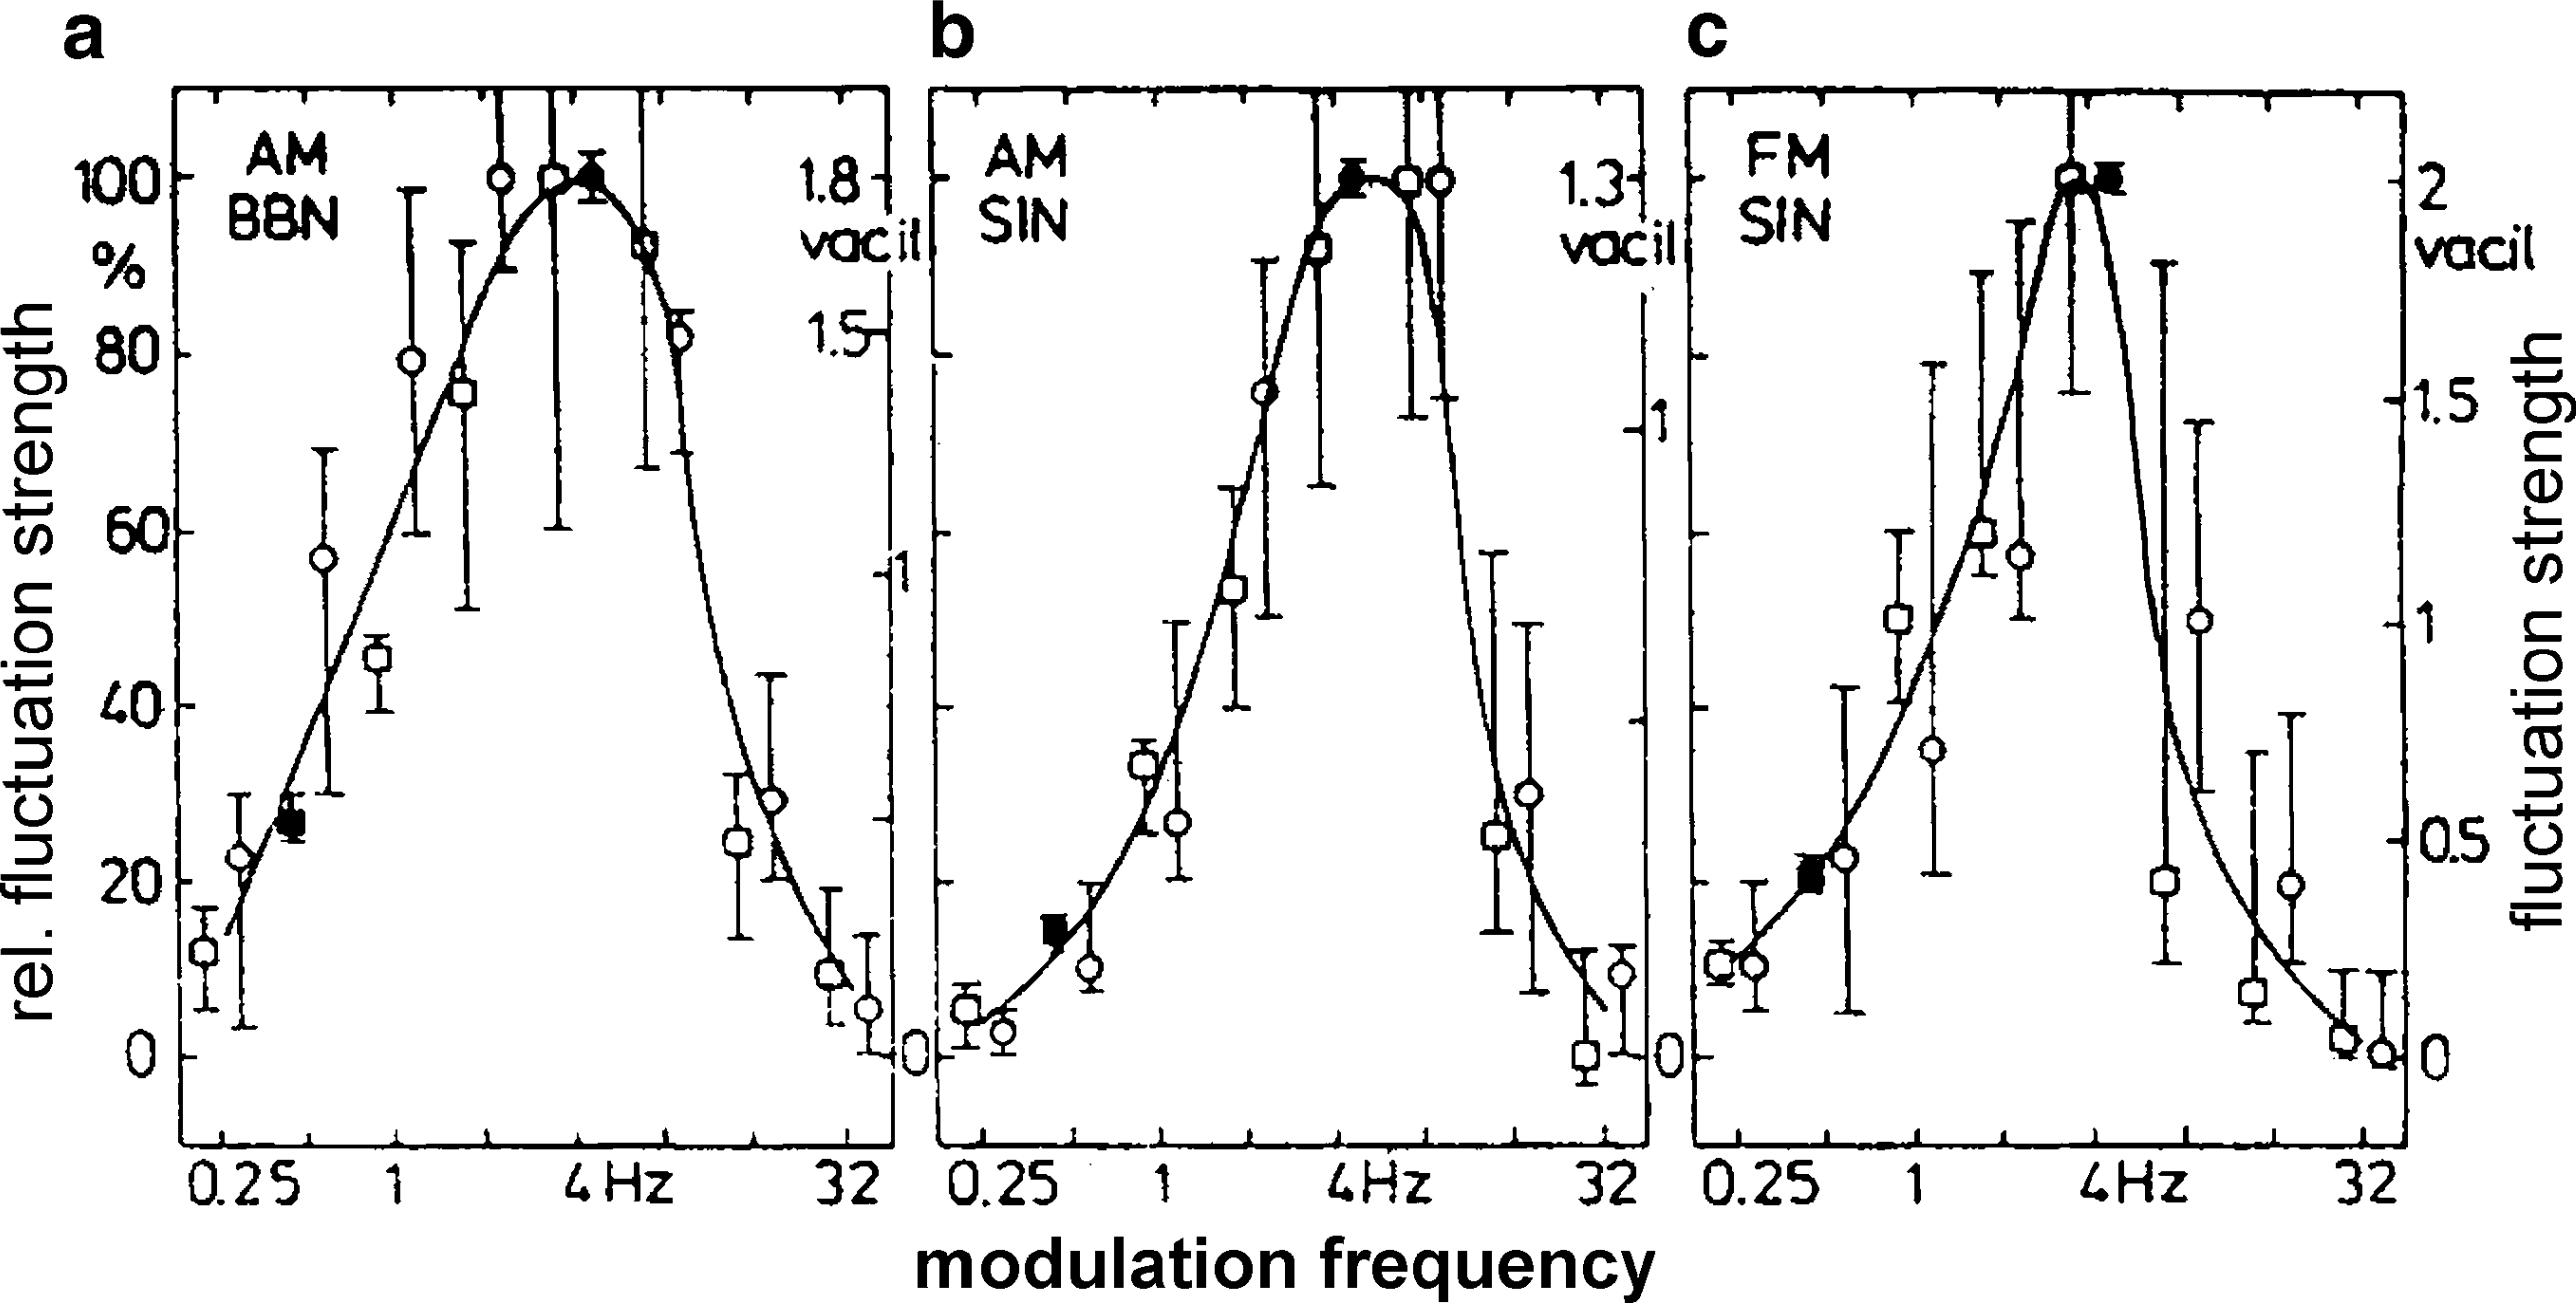
\includegraphics[height=5cm]{FluctuationStrengthVsModulationFrequency}
  \caption{Fluctuation strength as a function of modulation frequency for (a)
    amplitude-modulated broad-band noises, (b) amplitude-modulated tones and (c)
    frequency-modulated tones~\cite[pp.~248]{Fastl2007Psychoacoustics}}
\label{fig:flucstrenvmodfreq}
\end{figure}

It seems that a relation between fluctuation strength and speech production
exists, as the normal production rate of syllables during normal conversation
speed is about 4 syllables/second. This coincides with the frequency in which a
maximum value of fluctuation strength occurs (4 Hz).

Regarding sound pressure level (SPL) and fluctuation strength,
\cref{fig:flucstrenvsndpreslvl} shows their relation for two different stimuli
(tones and broad-band noise) and two modulation techniques (amplitude modulation
and frequency modulation). An increase in SPL entails an increase of fluctuation
strength, this being stronger when using amplitude-modulation.

\begin{figure}
  \centering
  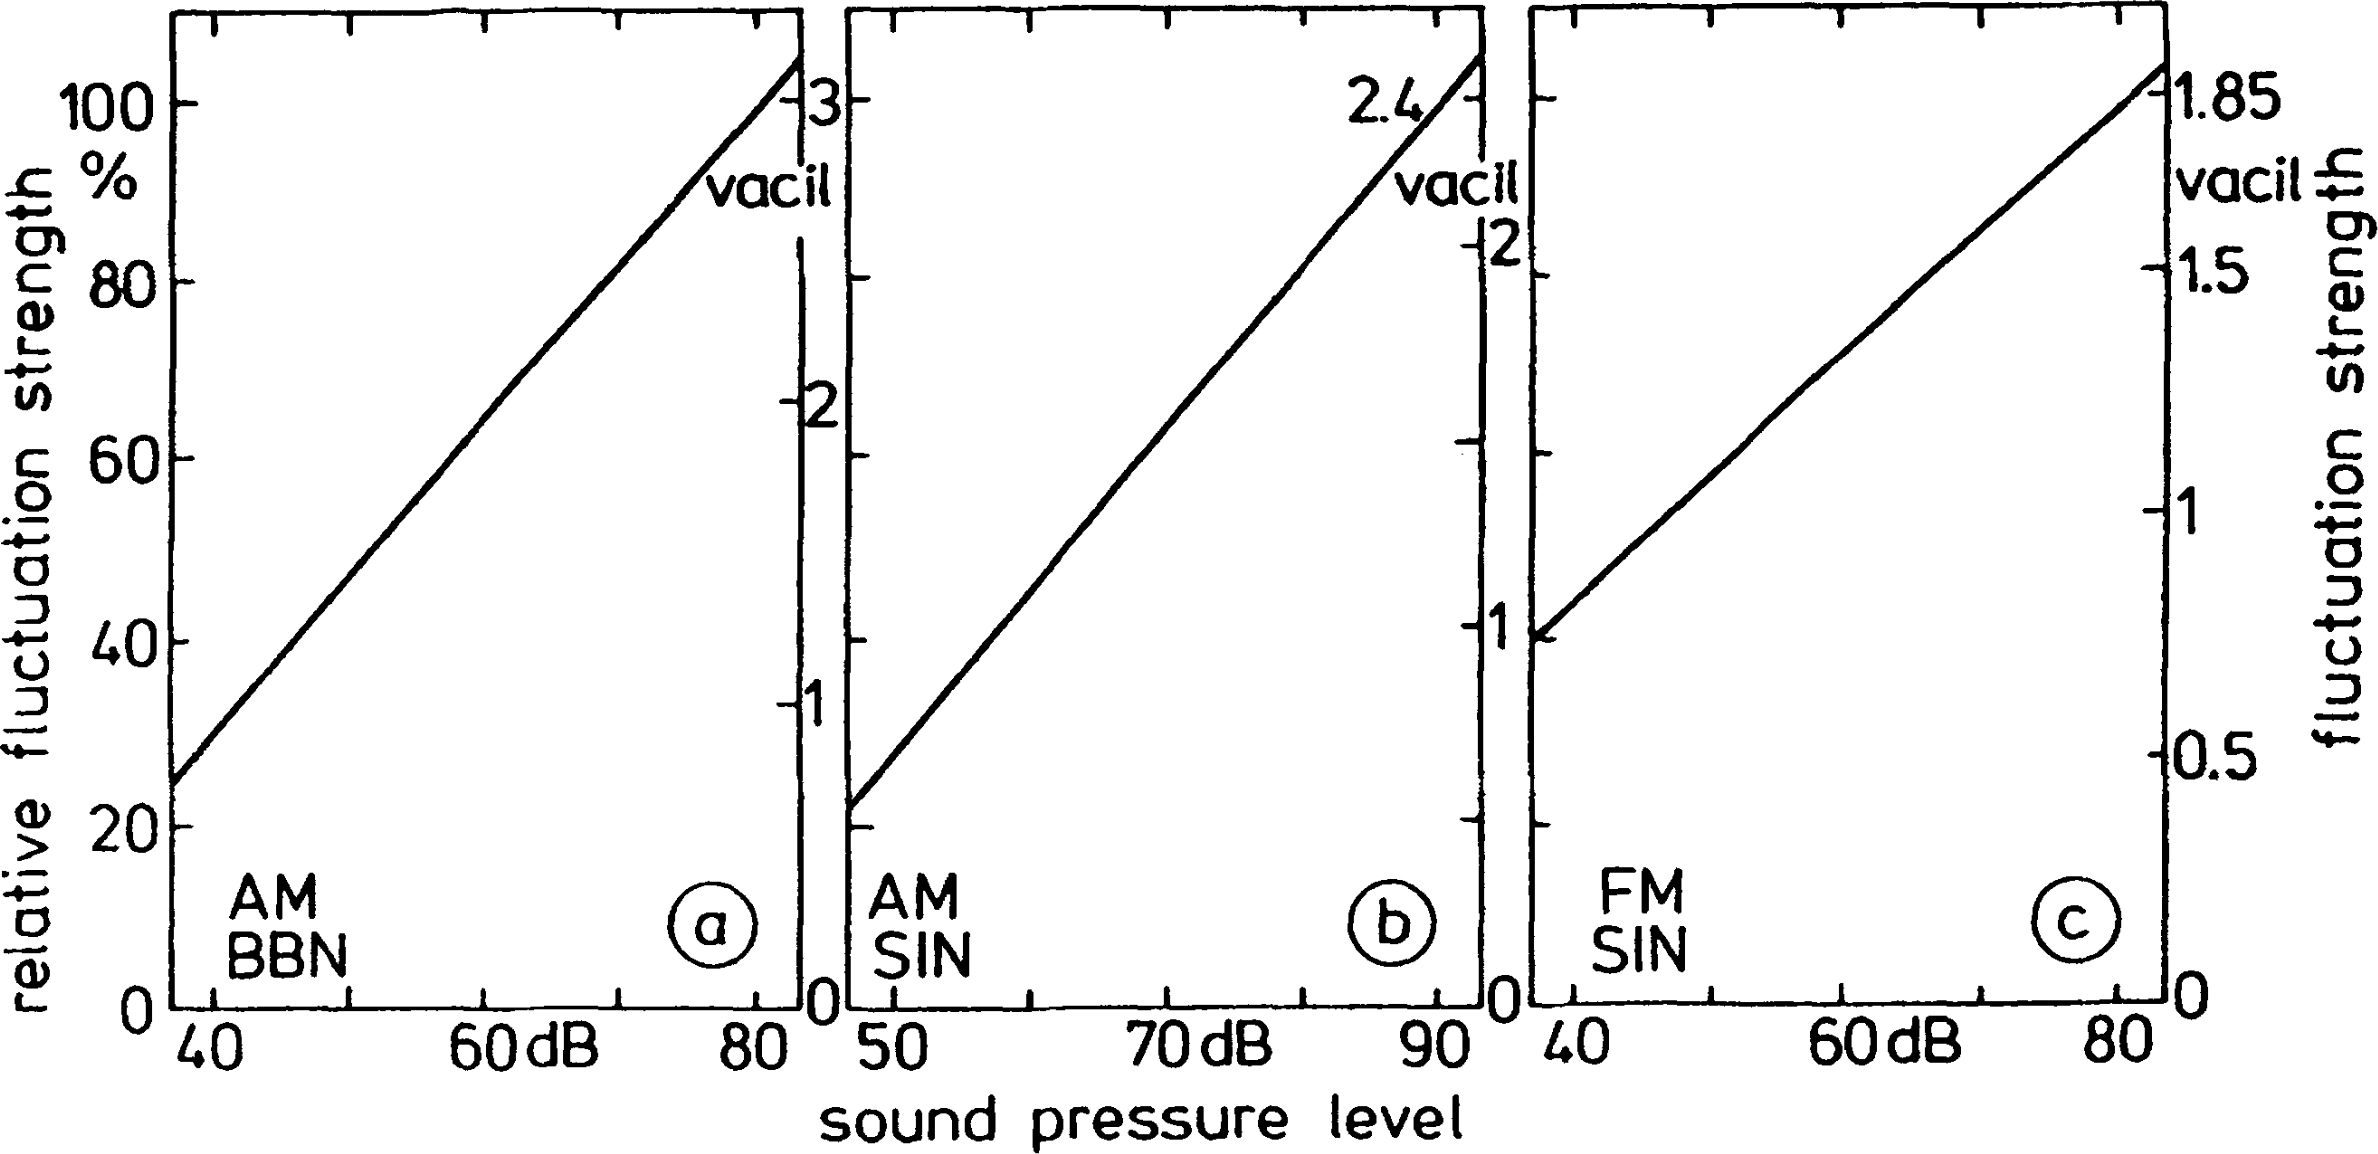
\includegraphics[height=5cm]{FluctuationStrengthVsSoundPressureLevel}
  \caption{Fluctuation strength as a function of sound pressure level for (a)
    amplitude-modulated broad-band noises, (b) amplitude-modulated tones and (c)
    frequency-modulated tones; modulation frequency of
    4Hz~\cite[pp.~249]{Fastl2007Psychoacoustics}}
\label{fig:flucstrenvsndpreslvl}
\end{figure}

Next the effect of modulation depth on fluctuation strength is analyzed, which
can be observed on \cref{fig:flucstrenvsmoddep}. It can be observer than,
between 3 dB and 30 dB the relation between fluctuation strength and modulation
depth is somewhat linear. After reaching a maximum value at around 30 dB, which
corresponds to a modulation factor of 94\%, fluctuation strength remains
constant with further increments of modulation depth.

\begin{figure}
  \centering
  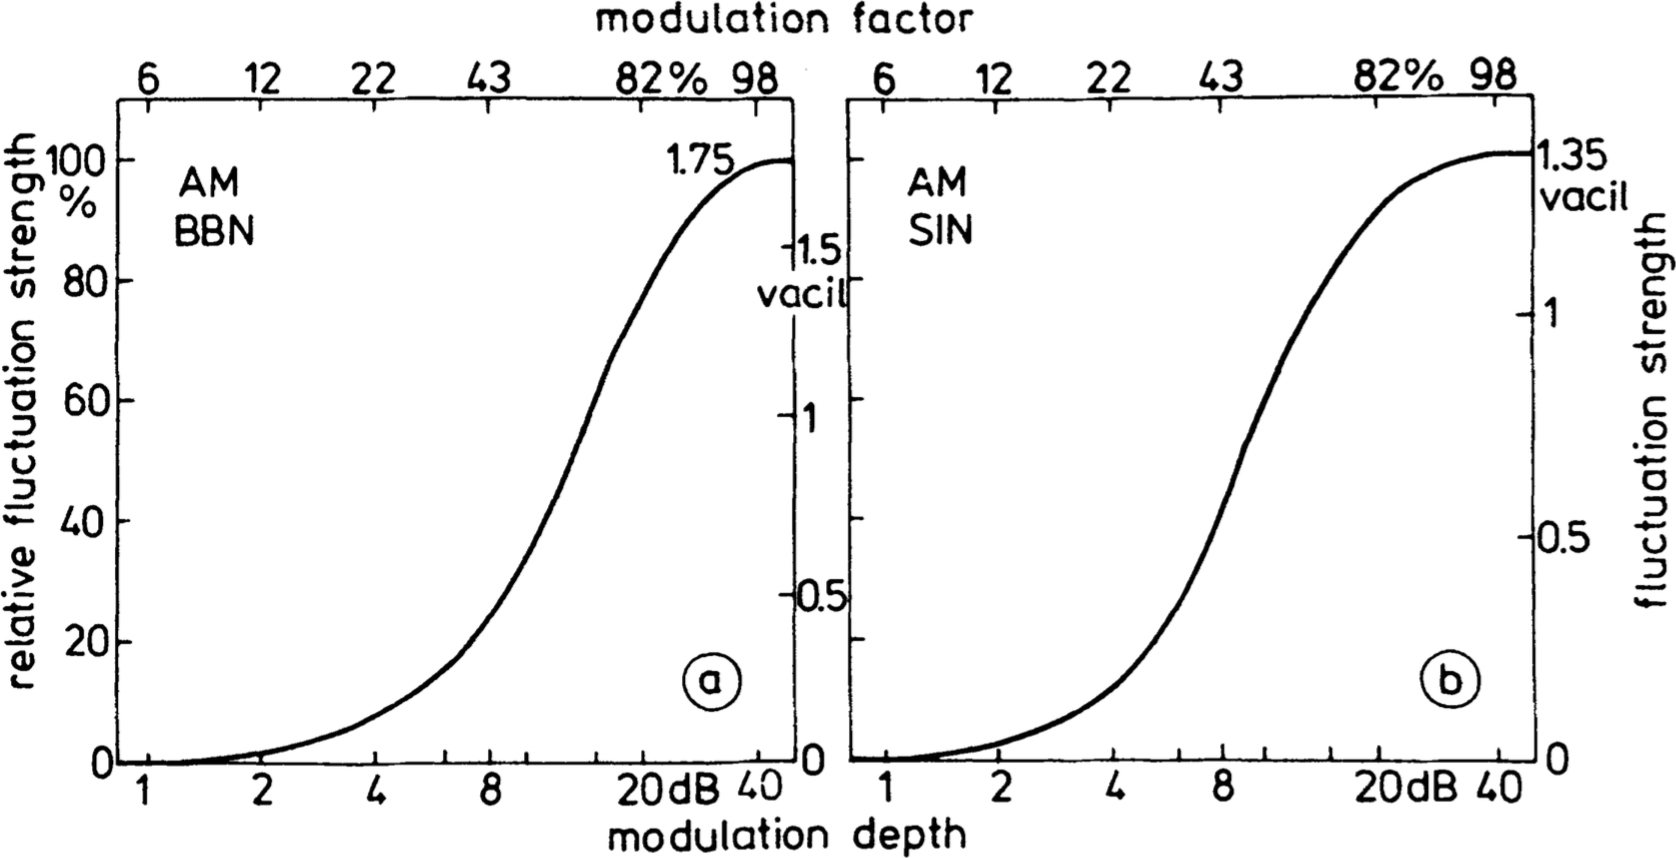
\includegraphics[height=5cm]{FluctuationStrengthVsModulationDepth}
  \caption{Fluctuation strength as a function of modulation depth for (a)
    amplitude-modulated broad-band noises of 60 dB SPL and (b)
    amplitude-modulated tones of 70 dB SPL and 1 kHz frequency; both with a
    modulation frequency of 4 Hz~\cite[pp.~249]{Fastl2007Psychoacoustics}}
\label{fig:flucstrenvsmoddep}
\end{figure}

\Cref{fig:flucstrenvscfreq} shows the relation between the center
frequency and fluctuation strength. Here a clear difference exists between the
type of modulation used. For amplitude-modulated tones there is a small
variability in the fluctuation strength, implying this a very little dependence
of the modulation frequency on fluctuation strength. For frequency-modulated
tones a clear dependence between both variables exists. For modulation
frequencies below 1 kHz the fluctuation strength is almost constant; above 1 kHz
it experiences a linear decrease until it fades away.

\begin{figure}
    \centering
    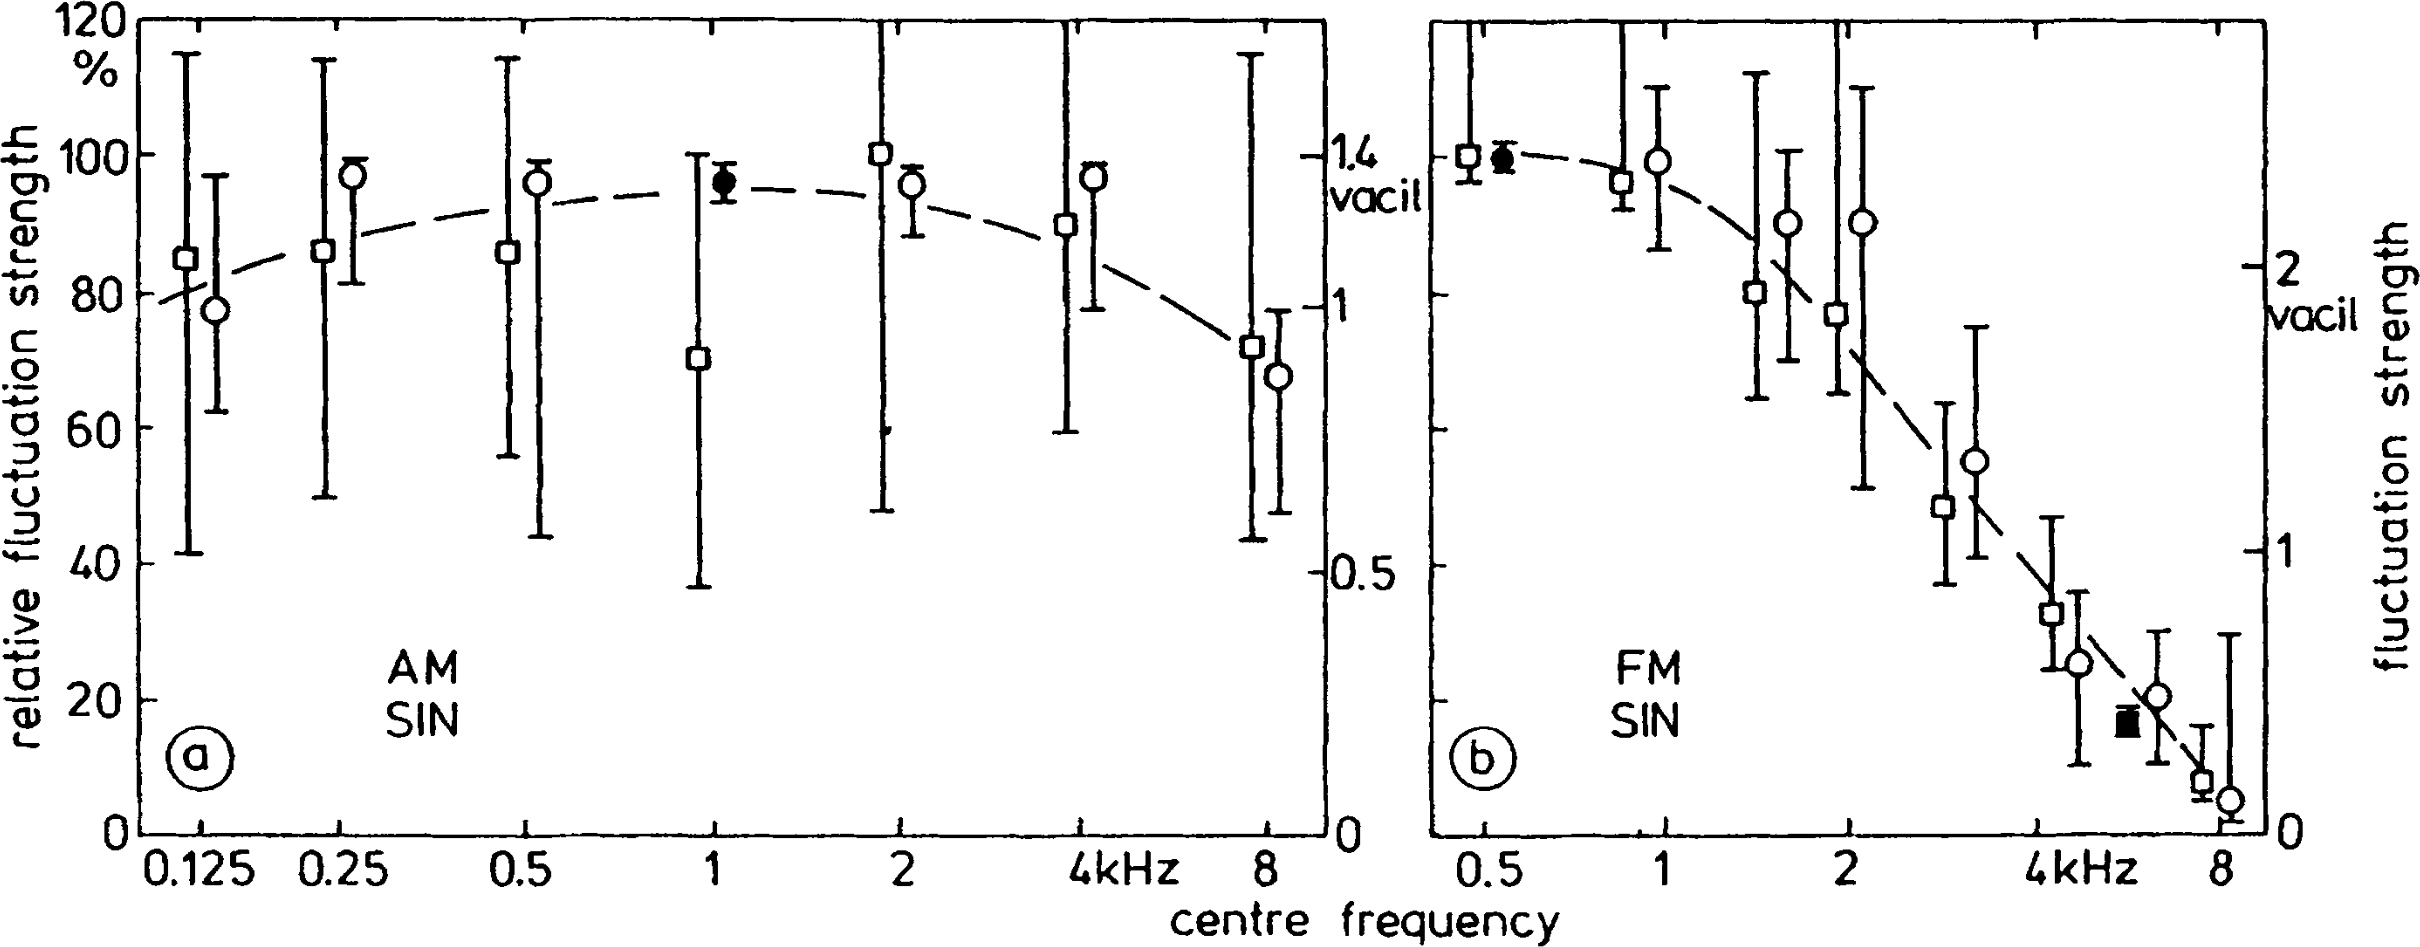
\includegraphics[height=5cm]
        {FluctuationStrengthVsCenterFrequency}
    \caption{Fluctuation strength as a function of center frequency for an
        amplitude-modulated tone of 70 dB SPL, 4 Hz modulation frequency and 40
        dB modulation depth (a), and a frequency-modulated tone with 70 dB SPL,
        4 Hz modulation frequency and $\pm200$ Hz frequency deviation
        \cite[pp. 250]{Fastl2007Psychoacoustics}}
    \label{fig:flucstrenvscfreq}
\end{figure}

To understand why this change of fluctuation strength occurs in the case of the
frequency-modulated tones, it is necessary to take into account the excitation
patterns that the modulated sounds cause regarding auditory filters. The
auditory filters are a series of overlapping bandpass filters that model the
frequency selective response of the auditory system. The excitation pattern
refers to the pattern that results as the outcome of all the precedent phases of
in the hearing process, being them the outer ear transmission, middle ear
transmission, and the auditory filters themselves.

In the case of fluctuation strength, for a 0.5 kHz tone the frequency would vary
between 300 and 700 Hz, this corresponding to a 3.5 Bark interval. For a 8 kHz
these values would be 7.8 kHz and 8.2 kHz, leading to a 0.2 Bark interval. The
proportion between these two is 17.5, which seems to be also the proportion
between the relative fluctuation strength for these two frequencies. Thus, this
leads to the idea that fluctuation strength can be explained in terms of the
excitation patterns that present themselves across the auditory filters.

Regarding fluctuation strength and frequency deviation, figure
\ref{fig:flucstrenvsfreqdev} depicts the relation between these two variables.
It can be seen that, after a frequency deviation of 20 Hz, there is a linear
increase of fluctuation strength with frequency.

\begin{figure}
  \centering
  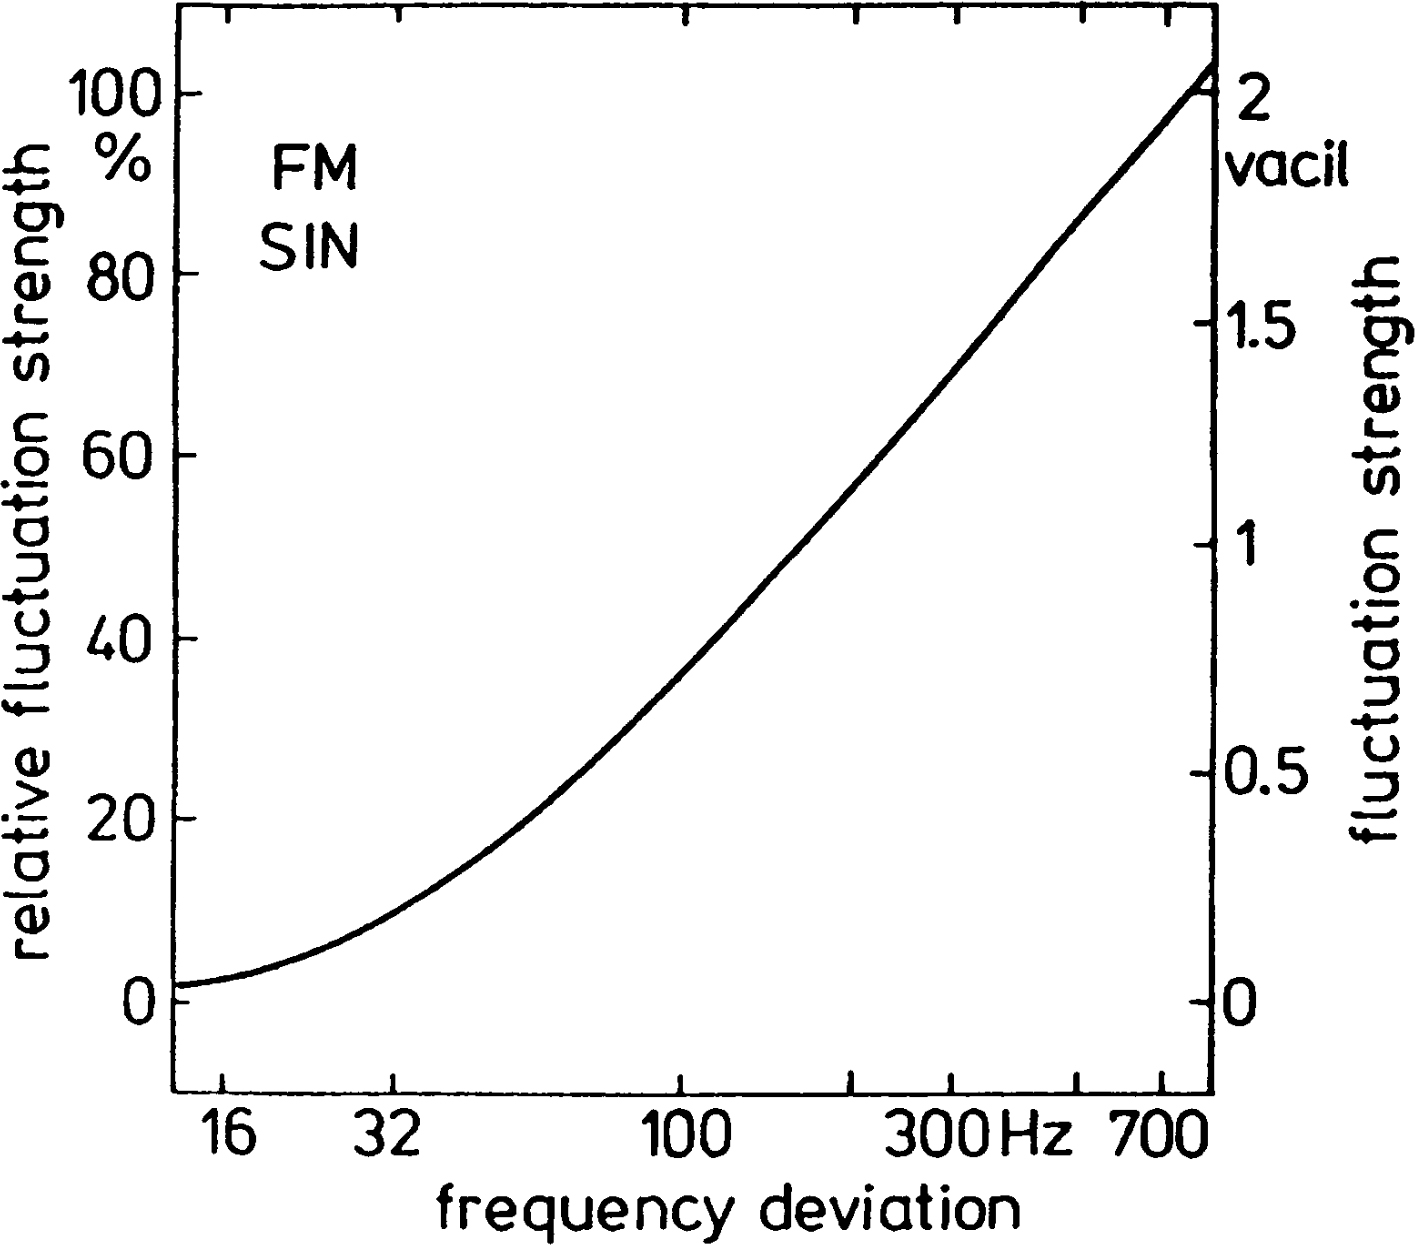
\includegraphics[height=5cm]
        {FluctuationStrengthVsFrequencyDeviation}
    \caption{Fluctuation strength as a function of frequency deviation for a
        tone with 70 dB SPL, 1.5 kHz center frequency and a modulation frequency
        of 4 Hz \cite[pp. 251]{Fastl2007Psychoacoustics}}
    \label{fig:flucstrenvsfreqdev}
\end{figure}

Another variable that affects fluctuation strength is the modulation index $h$
(also called modulation factor $m$). It is defined differently according to the
type of modulation used:
\begin{itemize}
    \item For amplitude-modulated signals is the ratio between the modulating
        signal amplitude $M$ and the carrier signal amplitude $A$,
        \begin{equation}
            h=\frac{M}{A}
        \end{equation}
    \item For frequency-modulated signals is the ratio between the maximum
        frequency deviation in the carrier signal ($\Delta f$) and the maximum
        frequency component of the modulating signal ($f_m$),
        \begin{equation}
            h=\frac{\Delta f}{f_m}
        \end{equation}
\end{itemize}

Then, regarding modulation index, it seems that a significant fluctuation
strength (10\% of the relative fluctuation strength, as defined by the authors)
is achieved with a modulation index that would correspond to about 10 times to
JND for modulation frequency. This would relate both the thresholds of
modulation frequency and fluctuation strength.

Not only modulated sounds can cause fluctuation strength, but also for non
modulated narrow-band noise. Figure \ref{fig:flucstrenvsbandwith} illustrates
this, where it can be seen that also at a 4 Hz frequency the maximum value for
fluctuation strength occurs. Regarding the SPL it behaves similarly as the other
sound sources.

\begin{figure}
    \centering
    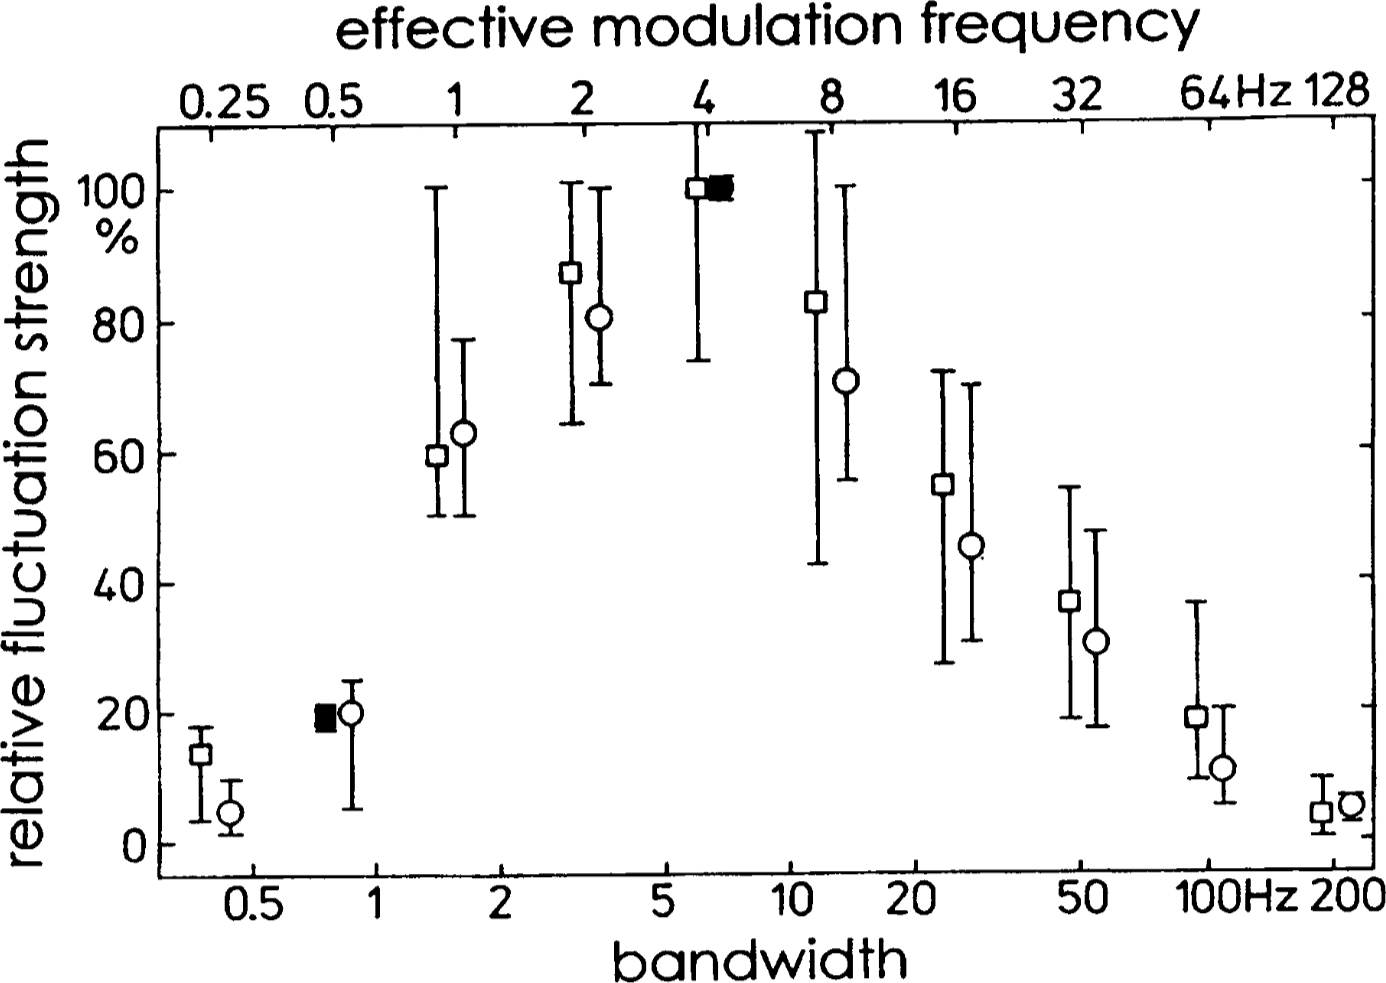
\includegraphics[height=5cm]
        {FluctuationStrengthvsBandwidth}
    \caption{Fluctuation strength as a function of bandwidth for non modulated
        narrow-band noise with 70 dB SPL and a center frequency of 1 kHz
        \cite[pp. 252]{Fastl2007Psychoacoustics}}
    \label{fig:flucstrenvsbandwith}
\end{figure}

Figure \ref{fig:flucstrensnds} compares the fluctuation strength of several
sounds, which physical characteristics are described in Table
\ref{tab:flucstrensnds}. The sounds that present the largest fluctuation
strength (1 and 2) can be related by the fact that they excite a large range of
frequencies taking into account the auditory filters. As so, it can be said that
fluctuation strength sums across critical bands.

\begin{figure}
    \centering
    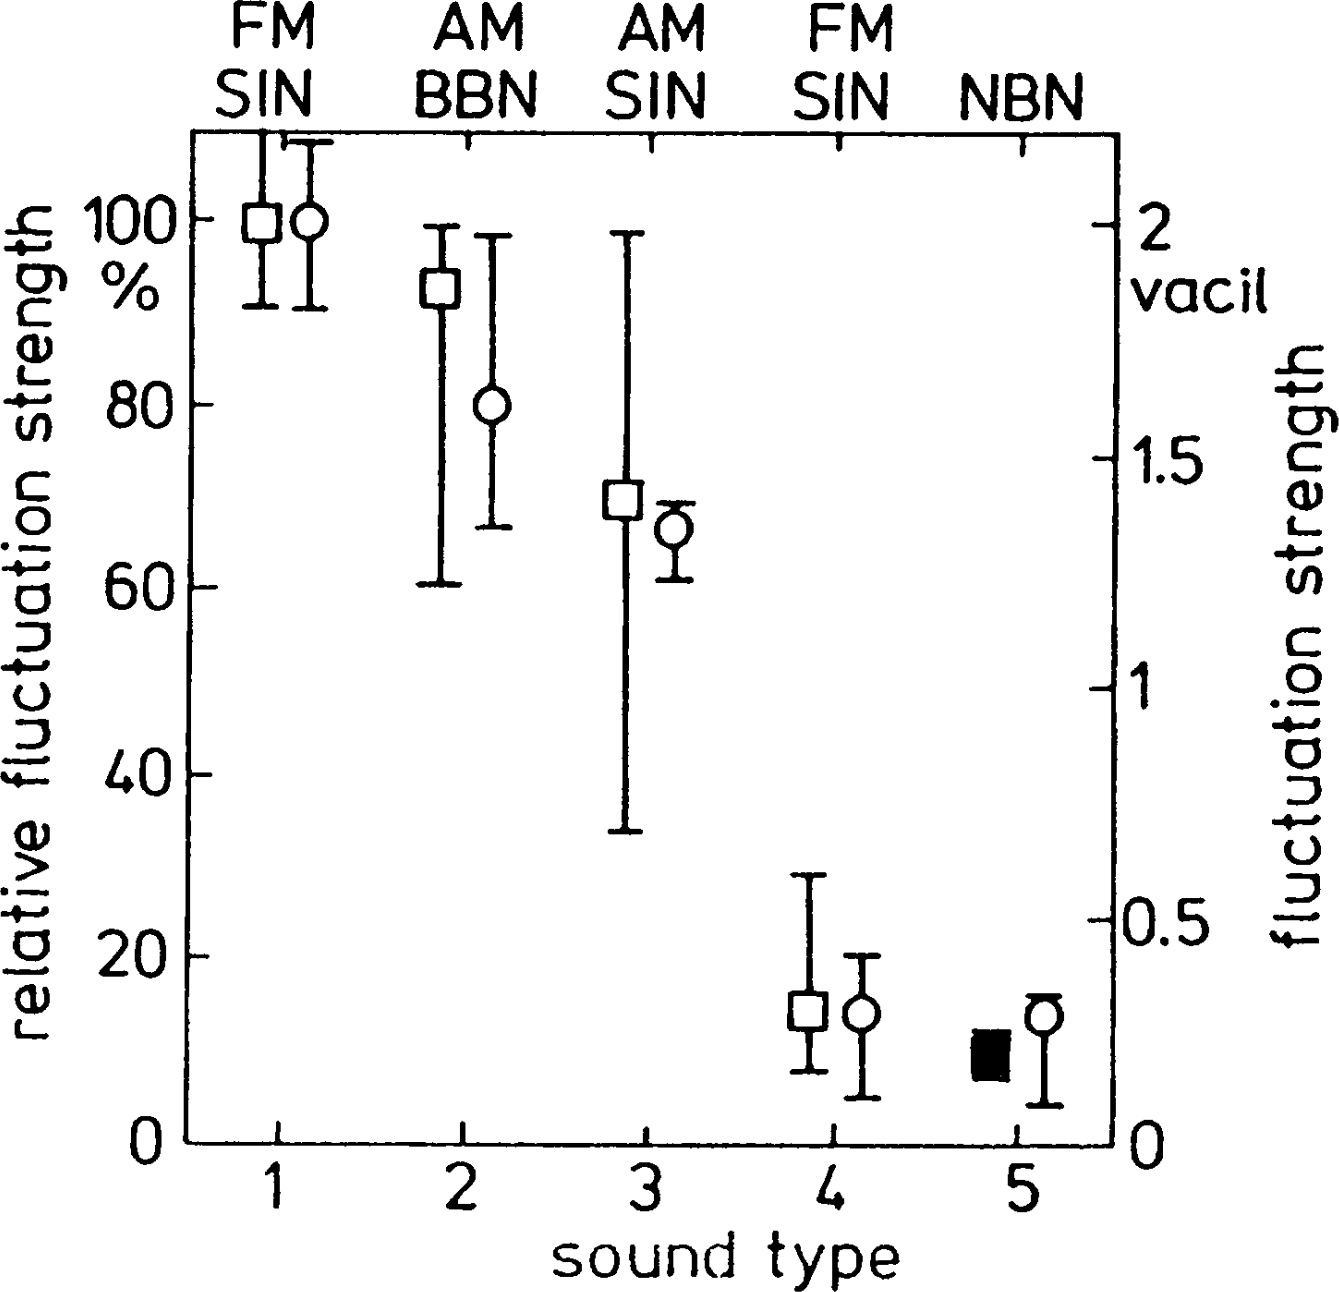
\includegraphics[height=5cm]
        {FluctuationStrengthSounds}
    \caption{Fluctuation strength of sounds 1--5 as described in Table
        \ref{tab:flucstrensnds} \cite[pp. 252]{Fastl2007Psychoacoustics}}
    \label{fig:flucstrensnds}
\end{figure}

\begin{table}
    \centering
    \begin{tabular}{ l r r r r r }
        \toprule
        Sound & 1 & 2 & 3 & 4 & 5 \\
        \midrule
        Abbreviation & FM & AM & AM & FM & \\
        & SIN & BBN & SIN & SIN & NBN \\
        Frequency [Hz] & 1500 & --- & 2000 & 1500 & 1000 \\
        Level [dB] & 70 & 60 & 70 & 70 & 70 \\
        Modulation frequency [Hz] & 4 & 4 & 4 & 4 & --- \\
        Modulation depth [dB] & --- & 40 & 40 & --- & --- \\
        Frequency deviation [Hz] & 700 & --- & --- & 32 & --- \\
        Bandwidth [Hz] & --- & 16000 & --- & --- & 10 \\
        \bottomrule
    \end{tabular}
    \caption{Physical data of sounds 1--5
        \cite[pp. 253]{Fastl2007Psychoacoustics}}
    \label{tab:flucstrensnds}
\end{table}

\subsection{Model of Fluctuation Strength}

A basic model on the temporal variation of a masking pattern in shown on Figure
\ref{fig:flucstrenmodel}, where the temporal variation of the amplitude of the
masker, also called temporal masking depth, is denoted by the magnitude
$\Delta L$. The inverse of the time difference between peak corresponds to the
modulation frequency $f_{mod}$.

\begin{figure}
    \centering
    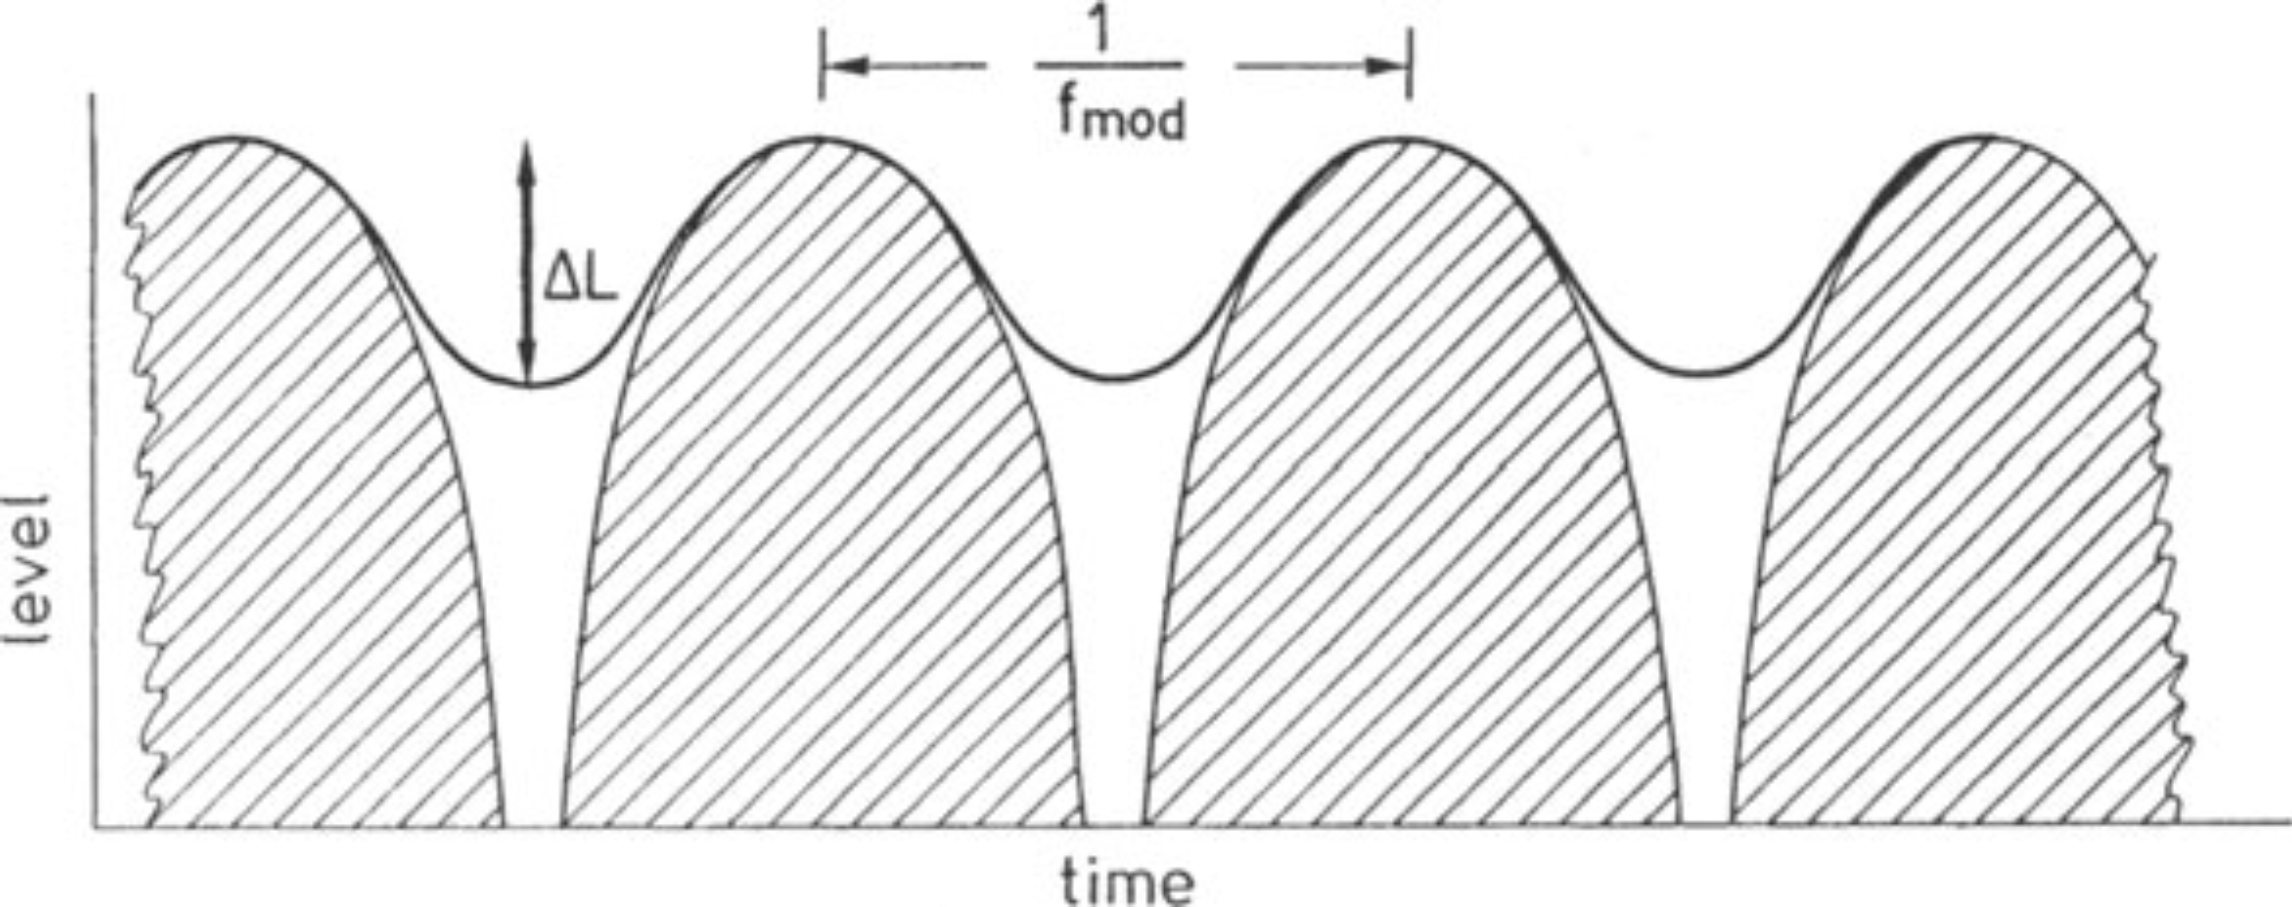
\includegraphics[height=5cm]
        {FluctuationStrengthModel}
    \caption{Model of fluctuation strength
        \cite[pp. 254]{Fastl2007Psychoacoustics}}
    \label{fig:flucstrenmodel}
\end{figure}

Equation \ref{eq:flucstrentempmaskmodfreq} shows the relationship between
fluctuation strength $F$, temporal masking depth $\Delta L$ and modulation
frequency $f_{mod}$, where the importance of the 4 Hz frequency is emphasized.

\begin{equation}
    F \sim \frac{\Delta L}{(f_{mod}/4\text{ Hz}) + (4\text{ Hz}/f_{mod})}
    \label{eq:flucstrentempmaskmodfreq}
\end{equation}

It is to note that there is dependency between the temporal masking depth
$\Delta L$ and the modulation frequency depending on the type of stimuli. In the
case of broad-band noise, temporal masking depth seems largely unaffected by
modulation frequency, whereas amplitude and frequency modulates tones these two
variable are dependent on each other, this being strongest on the frequency
modulated case. In order to address this, when modeling fluctuation strength
for these tones not a single $\Delta L$ value is taken, but instead it is
integrated across the critical-band rate scale.

Figure \ref{eq:flucstrentempmaskmodfreq} shows the resulting temporal masking
pattern for several values of modulation frequency. It can be seen that, as the
modulation frequency increases, the temporal masking depth decreases. This leads
to the idea that, although fluctuation strength presents a bandpass response
with respect to modulation frequency, the temporal masking suffers from a
low pass effect. It can be considered that the temporal masking depth decreases
linearly with modulation frequency.

\begin{figure}
    \centering
    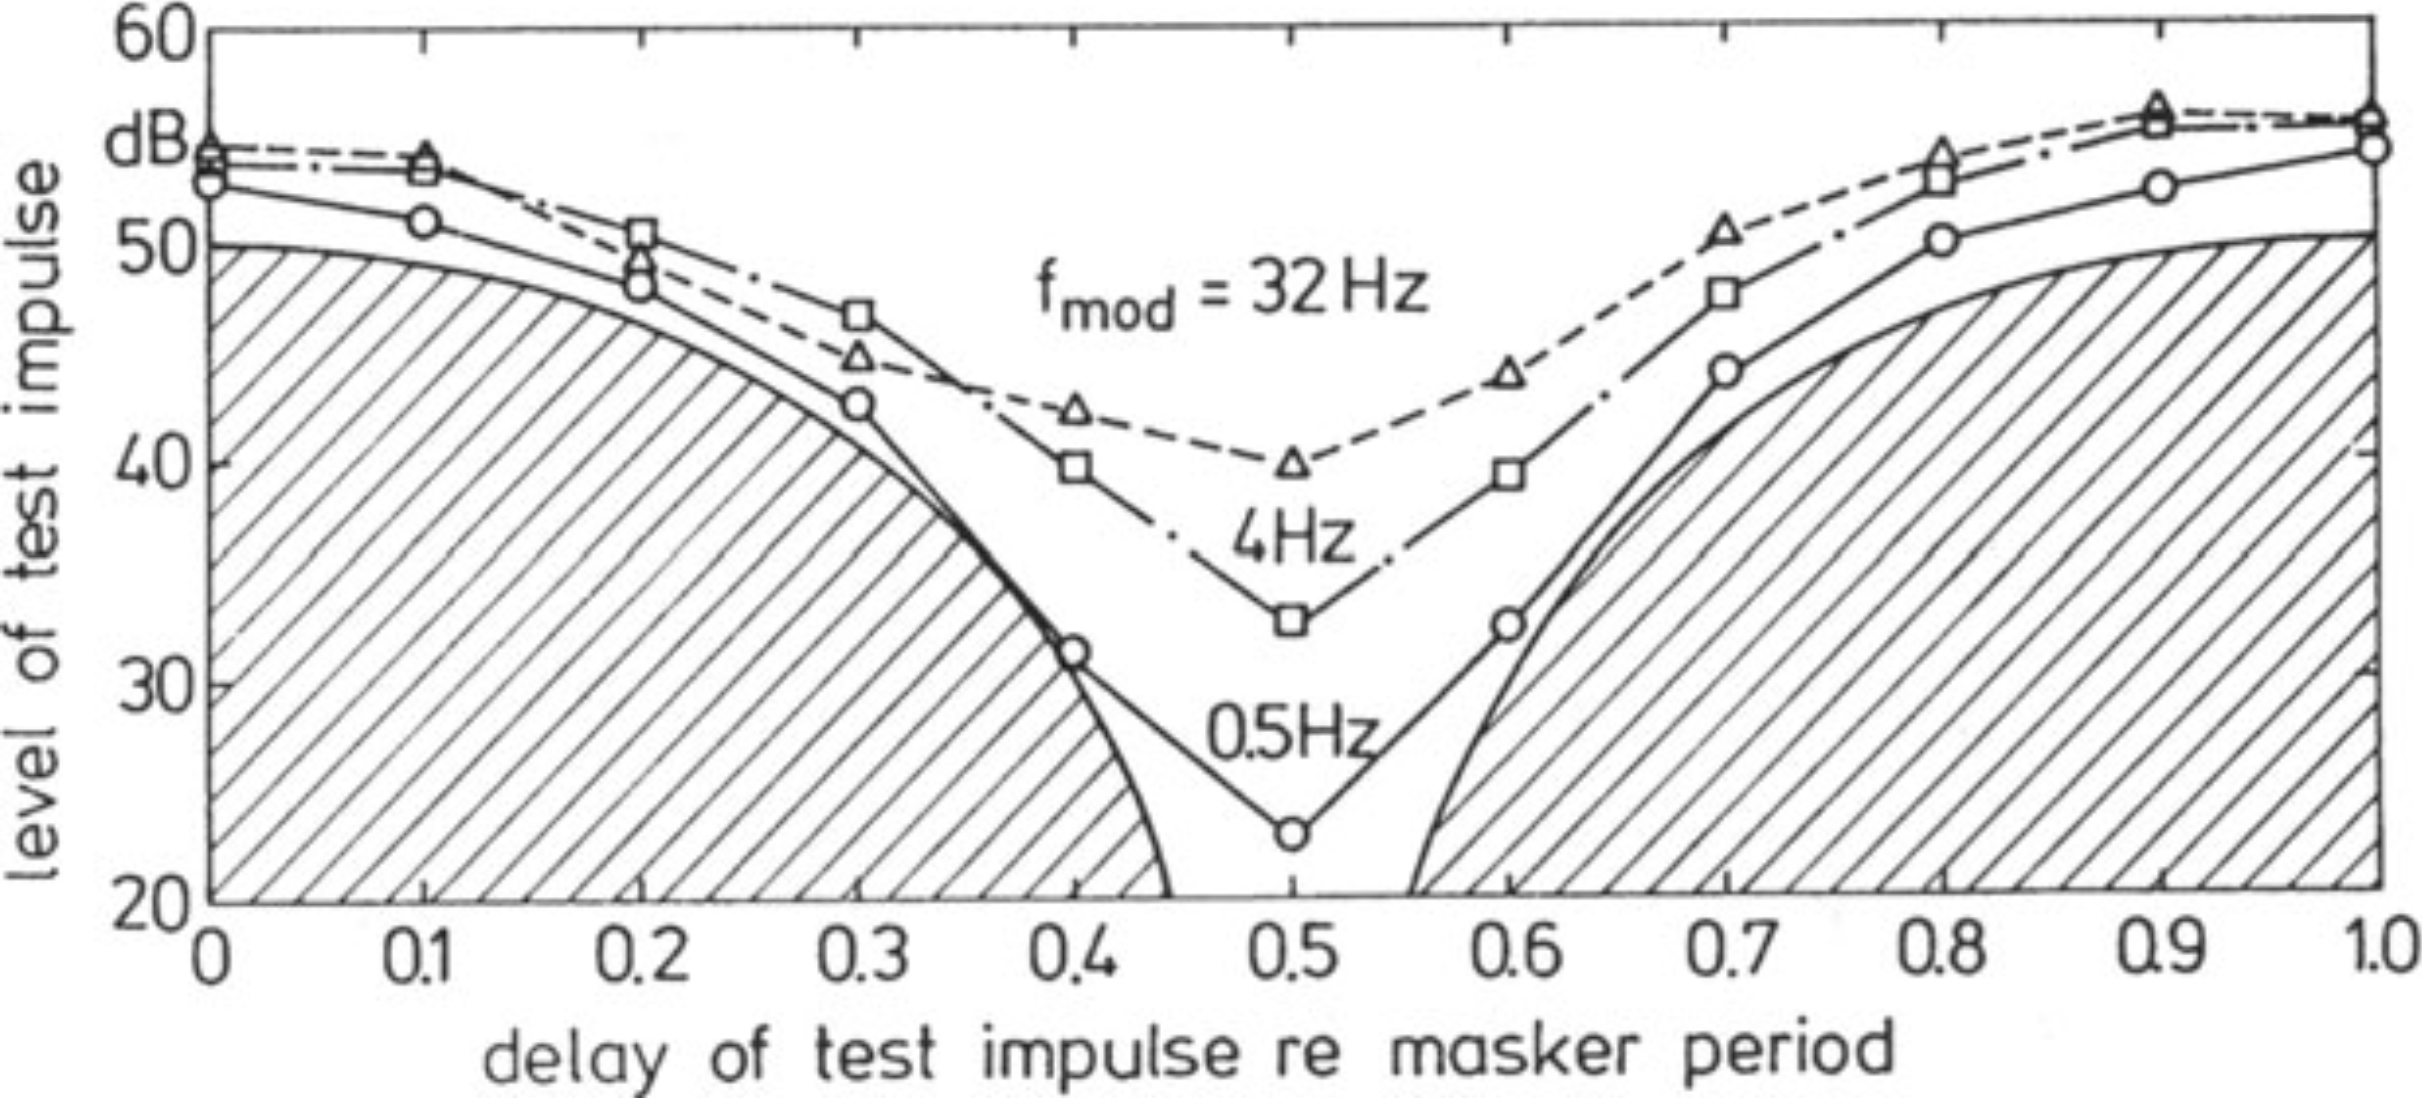
\includegraphics[height=5cm]
        {FluctuationStrengthTemporalMasking}
    \caption{Temporal masking pattern for an amplitude-modulated broad-band
        noise \cite[pp. 255]{Fastl2007Psychoacoustics}}
    \label{fig:flucstrenmasking}
\end{figure}

Taking all these into account, equation \ref{eq:flucstrenexbbn} presents an
updated model, in which $m$ is the modulation factor, and $L_{BBN}$ is the level
of broad-band noise. Similarly, equation \ref{eq:flucstrenexamfm} presents the
equivalent for the tone signals, where the temporal masking depth is integrated
across the auditory filters.

\begin{equation}
    F_{BBN} = \frac{5.8(1.25m-0.25)[0.05(L_{BBN}/\text{dB})-1]}
        {(f_{mod}/5\text{ Hz})^2+(4\text{ Hz}/f_{mod})+1.5} \text{ vacil}
    \label{eq:flucstrenexbbn}
\end{equation}

\begin{equation}
    F = \frac{0.008 \int_0^{24\text{ Bark}}(\Delta L/\text{dB Bark})\mathrm{d}z}
        {(f_{mod}/4\text{ Hz})+(4\text{ Hz}/f_{mod})} \text{ vacil}
    \label{eq:flucstrenexamfm}
\end{equation}

\section{Methods}

Absolute sensitivity accounts for the minimum level in which a stimulus is
detected. Differential sensitivity describes the extend to which changes between
stimuli can be detected. Sensory capability refers to what people actually hear,
and response proclivity refer to how people react to sounds.

\subsection{Classic Methods of Measurement}

\subsubsection{Method of Limits}

This method is used to determine the absolute sensitivity or the threshold for a
given sound characteristics. The experimenter is in control of the stimuli, and
the participant must state whether the stimuli characteristic is detected or
not. Several runs (presentations of stimuli with the physical characteristic
increasing or decreasing between presentations), alternating between ascending
and descending, are presented to the participants until the stimuli changes
status (detected to undetected, or the other way around). At the end, the mean
value of all the estimated thresholds is taken as the estimated global
threshold.

Responses biases may arise due to the anticipation of the threshold by
participants (since the run direction is known), or by habituation to the
stimuli, in this case reporting higher or lower values than the real threshold.

Step size between the stimuli can affect speed and reliability of the results.
A bigger step size allows faster experiments, but it is unreliable as it could
be not sensitive enough to detect the actual threshold. Smaller step sizes are
more effective in this regard but take more time of the experiment.

This method can also be used to determine differential threshold. In this case,
pairs of stimuli are presented, and the participant must state whether the
stimuli are equal or if one is greater than the other. One stimulus is keep as a
reference, while the other is varied, both in an ascending and in a descending
way. This gives three possible ranges of responses:
\begin{inparaenum}[(i)]
    \item stimulus A is greater than,
    \item stimulus B, stimuli are equal,
    \item stimulus A is lesser than stimulus B.
\end{inparaenum}
The range in which the stimuli are considered equal is called the interval of
uncertainty, and the just noticeable difference (JND) is usually taken as half
of this value.

\subsubsection{Method of Adjustment}

In this method the participant is in control of the stimulus, usually via a
continuous dial or knob. Then the participant must adjust the sound until it is
audible or inaudible, according to the stimulus starting point. The threshold is
then taken as the mean value of both values. In a differential setting, the
participant must adjust the stimulus strength until it matches the reference
stimulus strength.

This method can suffer from the persistence of stimulus bias, which results in
lower threshold when going in an downward direction and higher threshold when
going in an upward direction. To counteract this, both types of runs must be
used.

\subsubsection{Method of Constant Stimuli}

Similar to the method of limits, but in this case stimuli are presented in a
random order to participants. Then participants must state whether the stimulus
was detected or not. From the responses of all participants the psychometric
function can be obtained. The point where 50\% of the responses is achieved is
considered then the threshold.

In the case of a differential setting, pairs of stimuli are presented and the
participants must state whether the second stimulus was stronger or weaker than
the first (reference) stimulus. The point were the responses are at 50\% is
considered the point of subjective equality (both stimuli are perceived the
same), and the difference between the 50\% and the 75\% is the JND.

This method allows the placement of so-called ``catch trials'', i.e.\ trials
where there is no second stimulus present. This allows to control for guessing,
and reduces responses biases.

This method is more accurate than the other two methods, although is it usually
longer in duration. This can impact negatively participants, leading up to
fatigue and making it difficult for them to maintain motivation during the
experiment.

\subsection{Adaptive Procedures}

Adaptive procedures presents stimuli to the participants in one direction until
there is a change in participants answer; at that point then direction is
reversed until another change of answer is reached. It is said that adaptive
procedures converge to the threshold point, and make better use of trials by
placing most of them near the threshold itself.

\subsubsection{Bekesy's Tracking Method}

The direction of the change of the stimulus characteristic under study is under
control of the participant. For instance, in the case of loudness, the stimulus
begins with an inaudible level that is gradually incremented. As soon as the
participant starts hearing the stimulus he or she can push the button, that will
change the direction of the change to a decreasing one. While the button is
pressed, the change will continue downward. When the sound becomes inaudible
again, the participant can release the button, and the sound will start going
up again. In this way, the threshold can be tracked by the participant. This
procedure can lead to response biases in the cases which the stimulus change
rate is faster than the participant response rate.

\subsubsection{Simple Up-Down or Staircase Method}

This procedure is similar to the Bekesy's Tracking method, but in a discrete
way. Stimuli are presented sequentially either in a downward or upward direction
until a answer reversal occurs. In that case the direction is then reversed.
After six to eight changes of direction the method ends, and the 50\% point
value is calculated either with the mean value of the midpoints between changes
or with the mean value of all the peaks and troughs. As the stimuli are
presented in a sequential way, this can lead to response biases from the
participants, as they anticipate the stimuli that will be presented to them.
Also it is dependent of the step size, as the method of limits.

\subsubsection{PEST Procedure}

The parameter estimation by sequential testing (PEST) procedure is an adaptive
procedure that involves changes in direction and step size. When two consecutive
trials result in the same answer the step size is doubled. When a change of
answer occurs the step size of halved. When two consecutive changes of direction
occur the threshold is taken as the midpoint between these two values.

\subsubsection{BUDTIF Procedure}

The block up-down temporal interval forced-choice (BUDTIF) procedure is similar
to the PEST procedure. In this case blocks of stimuli are used instead of
individual ones. Also, instead of a yes-no response, a two-alternative forced
choice is used. Finally, it is possible to determine points in the psychometric
function other than 50\% by modifying the number of trials per block. For
instance, for a 75\% rate a block of 4 stimuli can be used, where if 3 out of 4
are classified correctly then the threshold is considered as the obtained value.
Otherwise the same procedure as the PEST is followed to alter the direction of
the trials, decreasing the stimuli intensity when four corrects responses are
obtained, and increasing them when there are less than three correct answers.

A variation of this procedure which utilizes a yes-no response also exists,
named the block up-down yes-no (BUDYEN) method. However, this method has the
disadvantage of not allowing to estimate false alarm responses, as a result of
the fact that pairs of stimuli are not used.

\subsubsection{Transformed Up-Down Procedures}

Simple Up-Down procedure converges only to the 50\% point in the psychometric
curves. By altering the criteria for increasing the stimuli level (up rule) and
decreasing the stimuli level (down rule), other points can be achieved. For
instance, by only decreasing the stimuli level when two consecutive positive
answer occur, the point to which the procedure converges is 70.7\%.

\subsection{Scales of Measurement}

Nominal scales refer to categorization of stimuli according to groups. Ordinal
scales imply that the values of the scale can be ranked, but a distance between
these values is not given. Interval scale specify both an order and a distance
among members of the scale; however, they do not specify a reference value or
zero. Lastly, ratio scale include a reference value, allowing to specify values
as ratios, expanding the amount of information conveyed by them.

There also exist three classes of scaling procedures. Discriminability (or
confusion) scales are generated by asking individuals to determine differences
between stimuli. Category (or partition) scales present the participant with the
task of dividing the stimuli range into equally spaced categories. Magnitude (or
ratio) scales ask individuals for an estimation of the ratio between two
stimuli.

\subsection{Direct Scaling}

\subsubsection{Ratio Estimation and Production}

Ratio estimation ask individuals to provide the relationship between to stimuli
in terms of the ratio between them. Ratio production allows individuals to
modify a given stimulus that must conform to a specific ratio, taking into
account the provided reference stimulus.

\subsubsection{Magnitude Estimation and Production}

Similar to the ratio estimation procedure, magnitude estimation ask individuals
to estimate a stimulus level taking as a reference an anchor value, usually
called a modulus. The modulus is assigned an specific value, for instance 10,
and the participant must state according to this reference value which would be
the value for the presented stimulus. For instance, a value of 60 would indicate
that the non-reference value is 6 times bigger than the reference value. An
alternative approach is to not include the modulus, in this case all the stimuli
are presented and the participant must assigned values to them taking into
account all of them. Magnitude production applies the same procedure but now the
participant must modify the non-reference stimulus level to comply with the
presented magnitude ratio.

Absolute magnitude estimation (AME) and absolute magnitude production (AMP)
do not include the reference value at all, neither they present stimuli in such
a way that a past stimulus can be used to assign the magnitude of a new one.

\end{theoreticalbackground}

\end{document}
